\section{Functional Requirements}
A nossa solução é  modular afim permitir a combinação de funcionalidades e a rápida extensabilidade. A \ref{fig:arch} explicita a arquitectura da nossa solução. Consultamos vários sites de feeds, extraimos os links para a notícia original, descarregamos a noticia, extraimos as entidades presentes e analisamos o sentimento de cada uma das frases da noticia e associamos esse sentimento à entidade de cada frase.
\begin{figure}[h!]
\centering
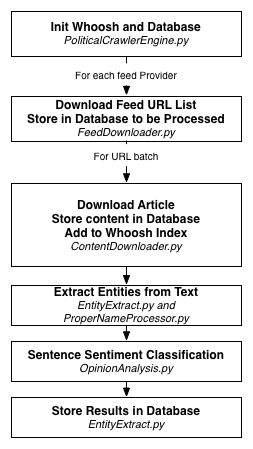
\includegraphics[width=0.25\textwidth]{./Figures/arch}
\caption{Arquitectura do Sistema}
\label{fig:arch}
\end{figure}
